\documentclass[11pt]{article}
\usepackage[top=1in, bottom=1in, left=0.5in, right=0.5in]{geometry}
\usepackage{graphicx}
\usepackage{url}
\begin{document}

\title{Analysing the project}

\author{Rahul Singhal 110050023,\\
	\texttt{rahuls@cse.iitb.ac.in}\\
	Shubham Lalwani Bharat 110050006,\\
	\texttt{shubham@cse.iitb.ac.in}\\
	Arun Prabhakaran 110050080,\\
	\texttt{arunp@cse.iitb.ac.in}}

\date{\today}

\maketitle

\section{Design Description}

The design broadly revolves around the concept that smoking kills.
A person goes for his cigarette and thus sets course to a chain of events which ultimately result in the man's head bieng chopped.
So much to make it interesting.\\

Well,the man pulls a string that is attached to a ball over a pulley.That ball strides up to hit another ball which is delibrately
placed in the previous ball's course.Now,the hit ball slips over the inclined platforms and pushes other balls placed en-route.
Finally,all these balls jump off the platform onto a hinged rod. Now,this hinged rod freely rotates about its hinge.
This rod was placed such that on it,lies precariously another ball.As soon as the moving balls fall on this rod(placed horizontally initially),
a projectile gets launched in the air.The trajectory of this projectile is so designed that it lands on another inclined platform.\\

The coefficiet of restitution of this platform is kept close to zero so as to not give the ball much  of a bounce.Now,this ball
continues to move on this platform and eventually hits a big T-shaped rigid body. Two balls ,placed beforehand on this body,
fall ahead (momentum conservation results in the rigid body toppling) over a platform containg dominoes. Down go all the dominoes,
one by one making each other fall.At the far end of the domino platform lies another ball.The last domino pushes this ball onta a weight 
(which originally is keeping two balloons in equilibrium).The falling of the ball flips over the weigtht thus freeing the balloons.\\

These baloons are assumed to be hydrogen filled with an inherent tendency to move against gravity.En-route freedom,one of them hits a ball,
which again has been precariously lying on a short flat portion. This short platforms runs over to an inclined one,
thus resulting in the ball gaining speed and moving over to a lightly placed bar on a support.The weight of the ball brings
about the flipping of this bar,thus freeing four small balls trapped by the bar head (the horizontal part of a L shape).These four balls 
then encounter one by one a gear system which is designed so as to distance them and thus bring forth the execution of the next part possible.\\

The design of this topmost level is the best and the most innovative part of the design.The first ball falls into a cup at the head of a
supported rod.This gives an impulse(angular) strong enough to fully rotate this rod and make it into an inclined path for the next ball.
This process goes on until the last ball falls through a system of tubes onto a hinged rod which simply chops off the head of the cigarette smoker.\\ 


\section{Interesting Points}

\begin{itemize}
\item First of all,our simulation succesfully,and hilariously, points out that smoking kills.It involves a plethora of innovative parts ranging from simple inclined planes to fully blown gears. 
 \begin{center}
 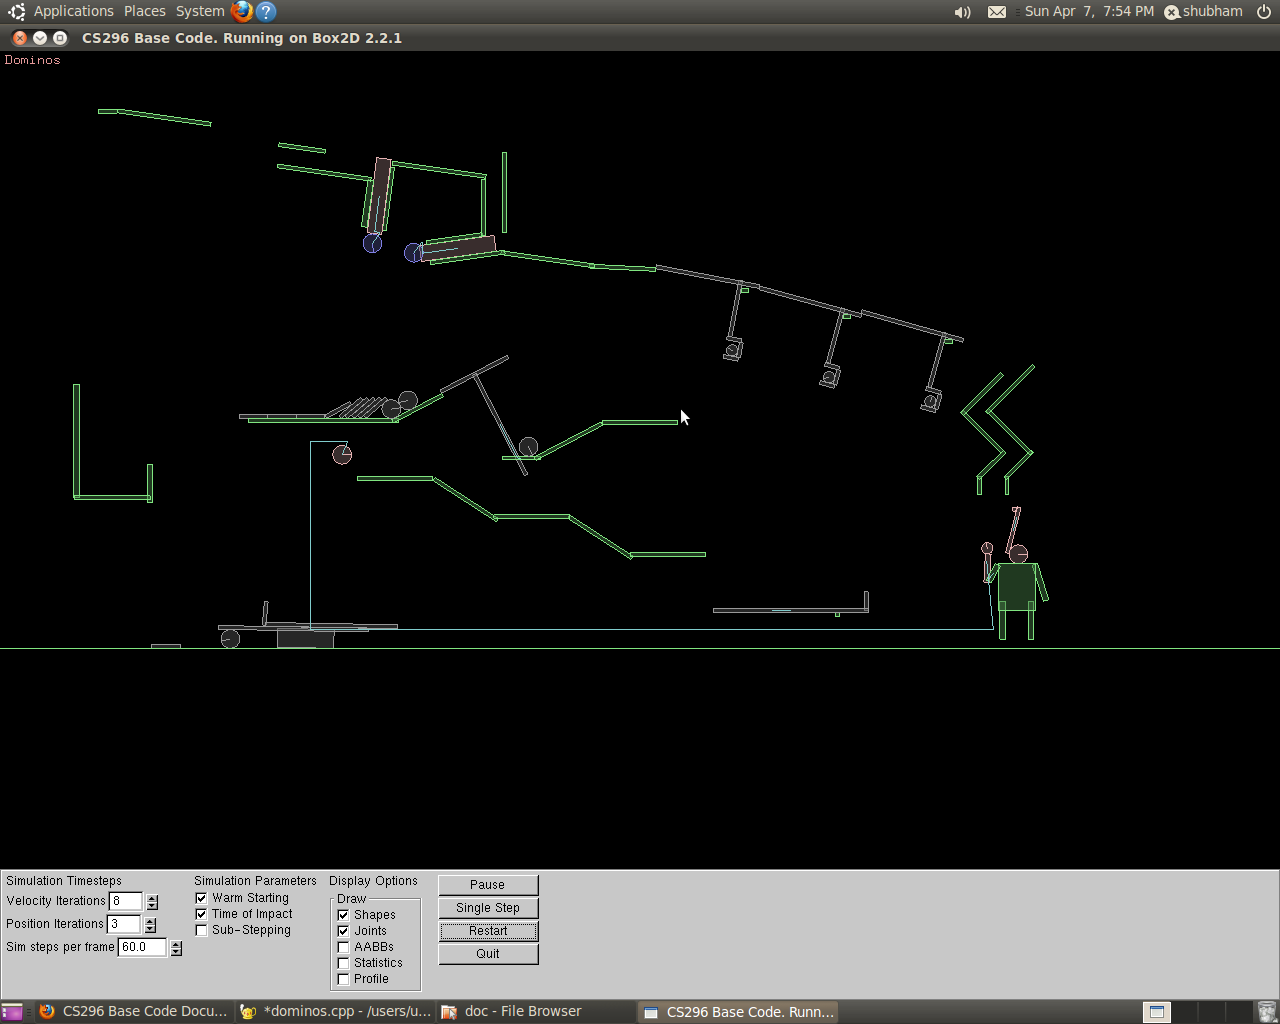
\includegraphics[scale=0.2]{images/I6.png}
 \end{center}
\item The most interesting part is the way in which we keep the four balls in the upper level of the simulation, at a distance optimum enough for the simulation to run smoothly.
 \begin{center}
 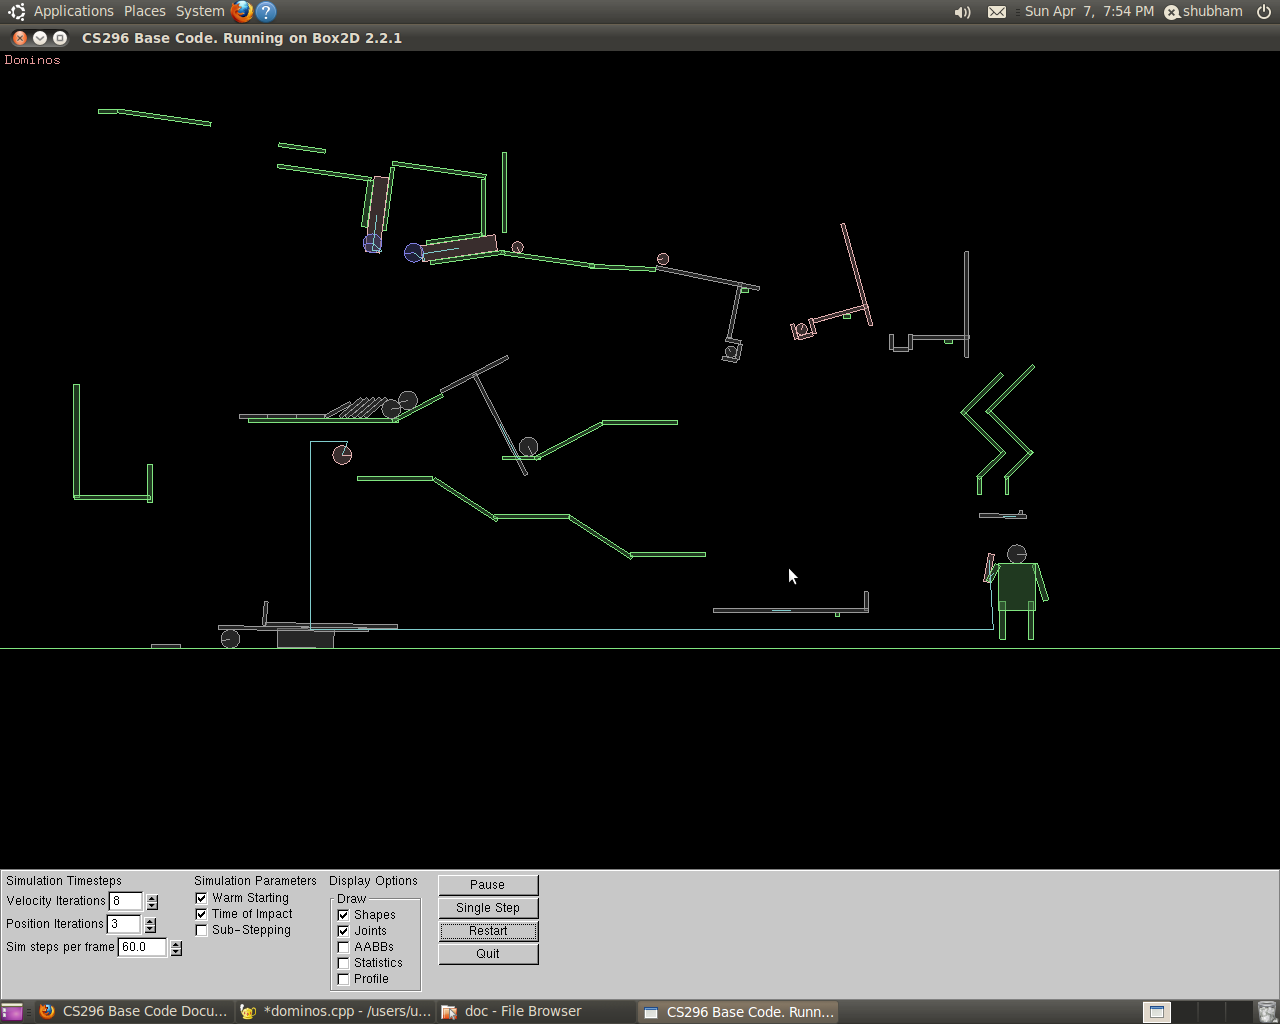
\includegraphics[scale=0.2]{images/I5.png}
 \end{center}
\item The viewer is guaranteed to look back and search for the slow moving fourth ball and sometimes,almost pine for it to get past the gears.
 \begin{center}
 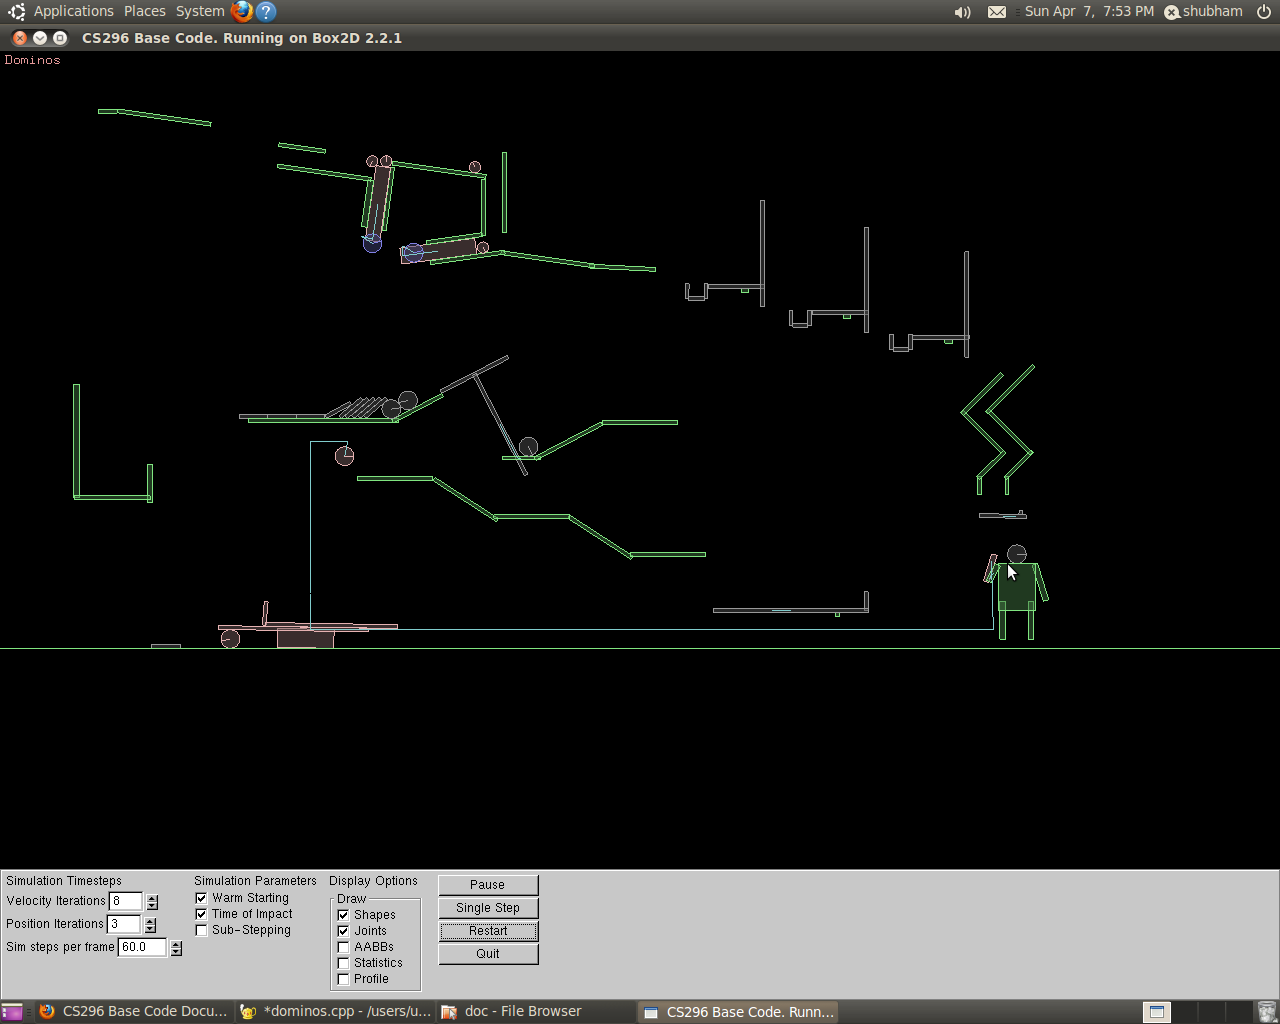
\includegraphics[scale=0.2]{images/I4.png}
 \end{center}
\item The physics use has been exhaustive and almost all physical laws make themselves useful in the simulation.Balloons and projectiles simply grace the innovation. 
 \begin{center}
 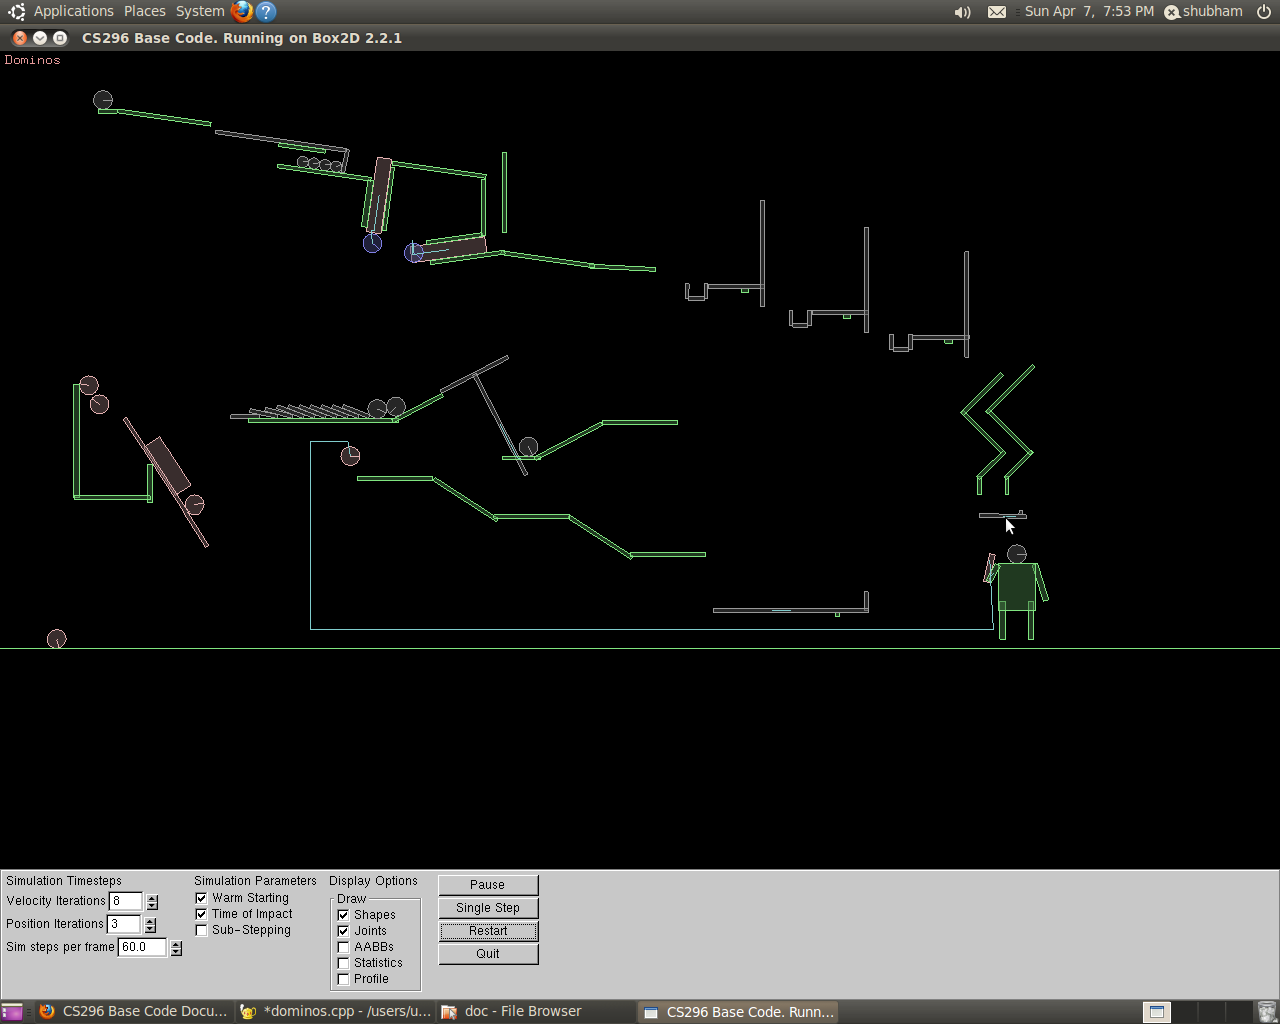
\includegraphics[scale=0.2]{images/I3.png}
 \end{center} 
\end{itemize}

\section{Deviation from actual design}

\begin{itemize}
\item The support for balloons involved a triangular shape but since we failed to follow the physcis in it we changed it to an L-shaped open box with support weight on the top to keep the balloons in equilibrium.
\item The T shaped structure on the second level does not contain boundaries as it was in the actual design. The balls on this platform are kept in such a way that the automatically remain in equilibrium.
\item The killing part had not been decided beforehand.Thus,the chopping of the head with an axe was newly introduced.
\end{itemize}

\section{Analysis of plots}

\subsection{Plot\_01}
The step time denotes the total time to complete a step in the virtual world(the step having been predefined in the real world as a fixed time).
The loop time includes various function calls (apart from those for iterations). The loop time increases inspite of the step time having decreased
becuase funcion calls form a major part in the loop time.The step time decreases beacuse the computer gets more efficient at performng the process
as it spends more time on it. 

    \begin{center}
   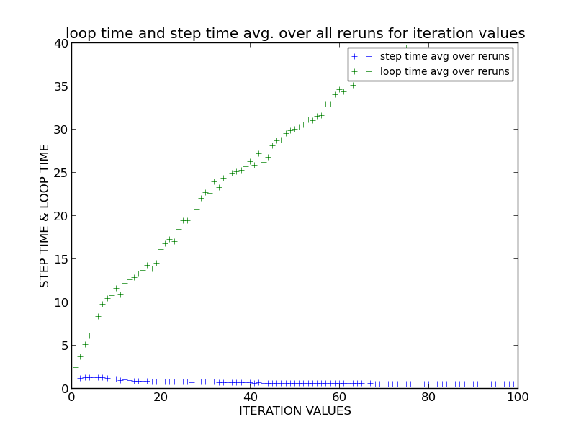
\includegraphics[scale=0.55]{images/g18_plot01.png}
    \end{center}
	
  \subsection{Plot\_02}
The step time is the sum of all the times involved(ie collision update,velocity update,position update etc.).This sum continuously decreases as the machine gets more efficient in doing the job as the time spent on the job increases(it assignes greater processing space ,and thus power to the problem taking this long a time).Also velocity updates involve working on the position data and then applying certain formulae to calculate velocity. Thus velocity update requires more time as compared to position updates.Velocity updates take place after considering collisions and the present state of the object.\\\\
Thus what we can conclude about the update process after taking in account the graph nature is, first position and collision updates take place and these result in velocity updates.
 \begin{center}
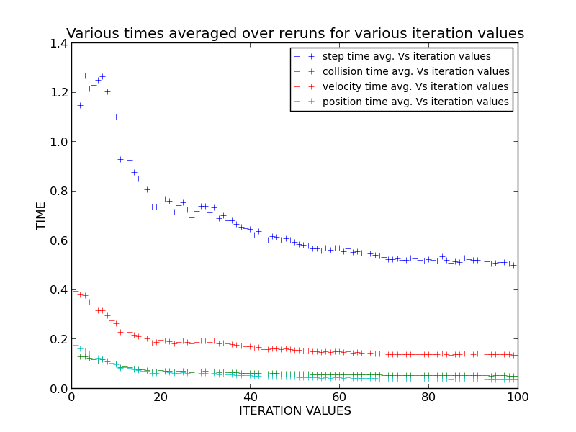
\includegraphics[scale=0.55]
{images/g18_plot02.png}
\end{center}

	
  \subsection{Plot\_03}
We  observe that a single rerun involves the whole iteration. What multiple reruns do is to simply average it(all the times) out.Obviously,every time the behaviour will be independent of the rerun happening(say first,second ,ninety-eight,etc.).Thus the graph.Loop times, still vary over reruns as they involve function calls which are the most uncertain,with respect to time.
 \begin{center}
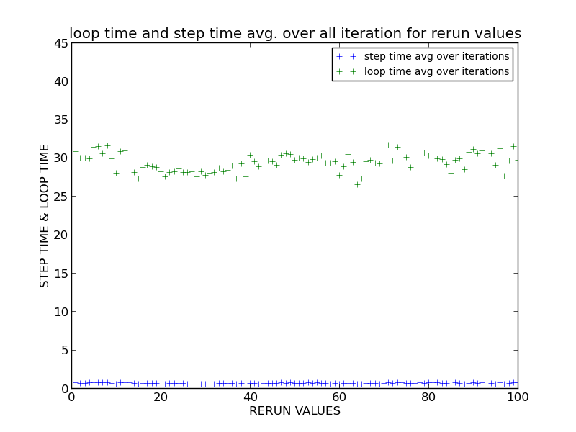
\includegraphics[scale=0.55]
{images/g18_plot03.png}
\end{center}
	
	
  \subsection{Plot\_04}
The similar analogy as that in the third plot regarding the independence of the values produced over an iteration and the rerun no. gives us that this graph should also be almost constant.Thus all the updates(position,velocity) and the collision time remain the same over all reruns, keeping the step time also same over all the reruns.
 \begin{center}
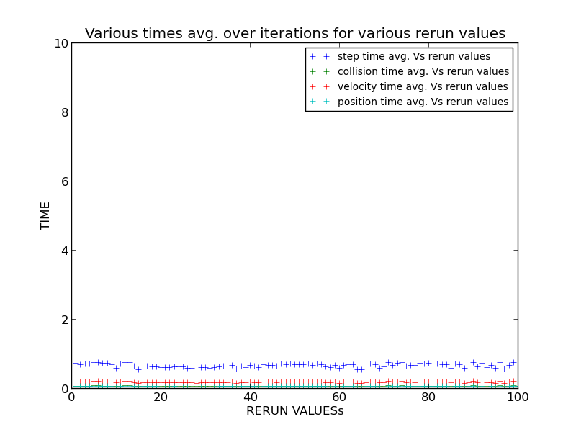
\includegraphics[scale=0.55]
{images/g18_plot04.png}
\end{center}
	
  \subsection{Plot\_05}
We observe that the errors decrease over the iterations as the system gets more proficient in getting step time as time progresses(since the system’s just freed resources also get diverted towards finding step time).Secondly,note that the error tends to decreases as the step time decreses(there is statistic proof for this even though the reason tends to become philosophical).
 \begin{center}
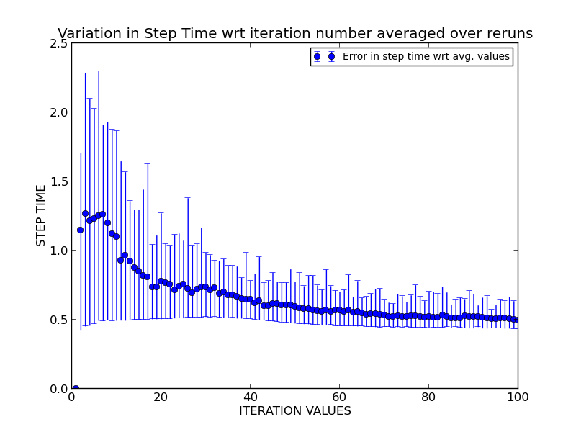
\includegraphics[scale=0.55]
{images/g18_plot05.png}
\end{center}
	
  \subsection{Plot\_06}
The step time decreases (self efficiency increasing systems!) over reruns(ignoring one arbitrarily high value at the end).The cumulative frequency (of loop time ) obviously increases.
 \begin{center}
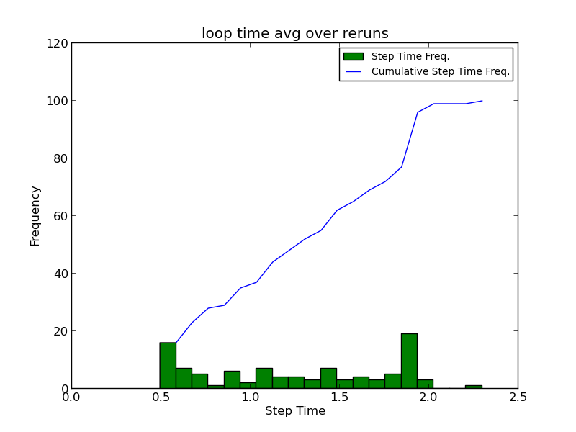
\includegraphics[scale=0.55]
{images/g18_plot06.png}
\end{center}

\subsection{Effect of System processes}
We tried to construct the same plots but under heavily loaded system conditions. I streamed a few youtube videos and played 3 movies in media player. As expected this took more time to generate the plots. A few observation we made from the plots are listed below:

\begin{itemize}
\item The process was slow and it took more than double time to produce the plots.To be more practical, the actual time for an execution under free conditions took 7.35 minutes and that under busy system conditions took 12.62 minutes to generate the plots.
All these times values were calculated using Linux command "time".
\item A somewhat vague observations was regarding the error bars in the 5th plot. The error bars in case of busy system conditions got elongated, showing more deviation from average value. We could not find anyy possible explanation for this result. This might be happening due to random system behaviour.
\end{itemize}

\subsection{Conclusion}

We have analysed all the graphs when the system was loaded and when it wasn't.

\section{Profiling}
This section gives an analysis of compilations profiling generated under different optimization being enabled. Basically our focus is on two types of build types:
\begin{itemize}
\item Release Mode
\item Debug Mode
\end{itemize}

Debug and Release are different configurations for building a project. As the name implies, one can generally use the Debug mode for debugging the project, and the Release mode for the final build for end users. The Debug mode does not optimize the binary it produces (as optimizations can greatly complicate debugging), and generates additional data to aid debugging. The Release mode enables optimizations and generates less (or no) extra debug data.

\subsection{The Process}
So what we have done to generate the data points in our program?\\
We compiled and ran our program once in debug mode and once in release mode configurations.We have decided to use the Linux utility "gprof" to profile the program.Based on the data in the sections below we have given a detailed inference that we drew after the data analysis. In addition we also generated the call and dependency tree using the python script "gprof2dot.py".


\subsection{Iteration Value}
We have chosen 10000 as the iteration value. When we tried for smaller iteration values like 100 , 1000 etc. , we did not get many concrete data points ie. only a few functions or method calls consumed all the process time. This left us with only a few profiled functions with a non-zero percentage in total process time while all the other functions ended up having zero or negligible process time percentage. \\
However we could have chosen a bigger iteration value but that would have increased the process time exponentially and we might end up with our machine hanged.Thus,all we are left with is a few range of iteration values(those which are neither too big nor too small) which produce a sufficient and easily profilable data.


\subsection{Debug Mode Observations}
As said earlier debug mode doesn't include any optimizations or most of the optimization options are turned off in this mode.So when we profile the data for compilation and program executation in debug mode,  we get a deep and very concrete data for various functions and operations being called during the process.\\

For instance, in our case "b2ContactSolver::SolveVelocityConstraints()" consumed the maximum percentage of time ie. 14.4\% for self calls and 30.6\% time including the calls it made to its descendants.

Below are a few functions that topped the list of time allotment :
\begin{itemize}
\item operator*(float, b2Vec2 const\&) [7.56\%]
\item b2Vec2::b2Vec2(float, float) [8.19\%]
\item b2ContactSolver::SolveVelocityConstraints() [14.4\%]
\end{itemize}

Below is the call graph for debug mode configuration data :
 \begin{center}

\includegraphics[scale=0.04]
{images/debug.png}
\end{center}
 As the width of the graph is too big, so we have scaled it down so that it fits in the page.To have a better look at the graph [debug.png] see the image file in the images folder.

 \subsubsection{Graph Interpretation}
We get a highly interlinked graph with loads of dependancies and one look at the graph gives us a good enough idea on the depth of the debug mode.Since no optimisation is done in the debug mode,we see a lot of nodes in multiple levels in the graph.\\
Every node in the graph represents three data units:
\begin{itemize}
\item The function name 
\item Percentage of time consumed for self calls
\item Total percentage of time consumed for the self calls and calls to its descendants.
\end{itemize}
The branches in the graph connect the parent node to a child node which depicts that the parent calls the child during its own execution.

\subsubsection{Conclusion}
Debug mode gives us an indepth insight of what is going inside the program and this is very well depicted by a long list of the profiled functions.This is the very reason why people use this mode to analyse and have a critical view of the program and thus improve on its loopholes and make it better.

\subsection{Release Mode}
This is the mode in which we compile when we release our program(outsourcing). In this mode,most of the optimisations are automatically enabled. We have added -O3 flags in the MakeFile to enforce the level 3 optimisation and produce a samll and faster executable. 

In release mode, the following functions significantly dominated the time taken :
\begin{itemize}
\item b2Distance(b2DistanceOutput*, b2SimplexCache*, b2DistanceInput const*) [24.14\%]
\item b2TimeOfImpact(b2TOIOutput*, b2TOIInput const*) [17.24\%]
\item b2ContactSolver::SolveVelocityConstraints() [13.79\%] 
\end{itemize}
\subsubsection{Graph Interpretation}

We see a cleaner and more consise graph due to the optimisations done under release mode.Below is the call graph for profiling data in the release mode:

 \begin{center}
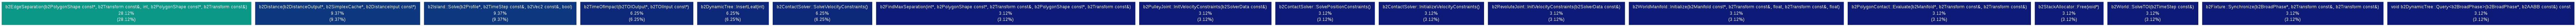
\includegraphics[scale=0.08]
{images/release.png}
\end{center}
The width of the graph being big,we have scaled it down so that it fits in the page.To have a better look at the graph [release.png] see the image file in the images folder.

\section{Few optimizations we observed}
\subsection{For loop unroll}
For loop unrolling means replacing the loop with actual code when the number of iterations is known.Basically it is a technique that attempts to optimize a program's execution with a trade-off on its size.\\
\begin{itemize}
\item Loops are re-written instead as a repeated sequence of similar statements.
\item -funroll-loops flag of the GNU C Compiler does this optimization.
\item The Bod2D file dominos.cpp contains some instances of such loops which can be improved.
\end{itemize}

\subsection{Variable Reuse}
Many times we need to use an object again and again in a code. But for every use of this object, we reference this object by a pointer and this takes time, thus effecting the efficiency. \\
So it is better to make a temporary copy of this object and use this temporary object instead.\\
We found a few variables in the Box2D files b2CollideEdge.cpp and b2CollidePolygon.cpp that referenced objects that were actually constructed in some other file.So this is an instance which can be improved upon.

\subsection{Inline functions}
This is basically an optimisation which replaces a function call with its actual code and thus prevents a lot of pointer referencing and kepng a check on the size of the execution stack of functions.\\
Functions like operator* , operator- etc. can be made inline.

\section{Conclusions}
We have analysed the graphs of lab05 and inferred them the best we could.\\
We have seen both the modes of build and analysed their pros and cons.We have also briefly analysed the optimisations involved.

\bibliography{references}
\bibliographystyle{plain}
\cite{rollingBodies}
\cite{RubeGoldbergmachineWiki}
\cite{RubeGoldbergHome}
\cite{stackoverflow}



\end{document}

